\documentclass[a4paper, 12pt, english]{report}
\usepackage[utf8]{inputenc}
\usepackage{amsfonts}
\usepackage{graphics}
\usepackage[finnish]{babel}
\usepackage{titlesec}
\titleformat{\chapter}
{\Large\bfseries}
{}            
{0pt}      
{\huge} 

\newcommand{\topic}{My application to the board of AYY}
\usepackage{hyperref}
\hypersetup{pdfpagemode=UseNone, pdfstartview=FitH, colorlinks=true,urlcolor=red,linkcolor=blue,citecolor=black,pdftitle={\topic},pdfauthor={Onni Lampi}}
\setlength{\parindent}{0mm}
\setlength{\emergencystretch}{15pt}
\newcommand*{\findate}{\the\day.\the\month.\the\year}

\begin{document}



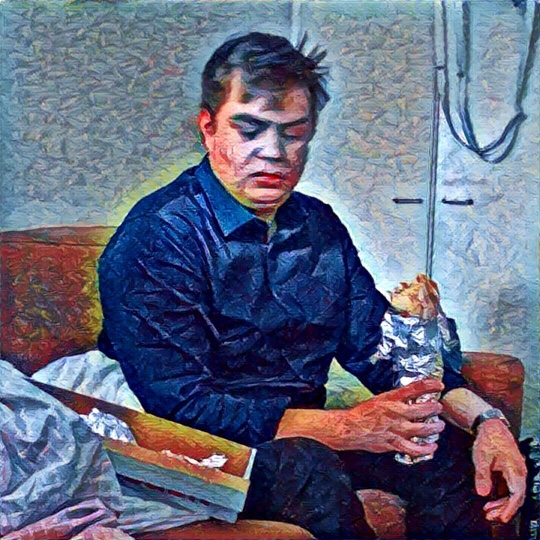
\includegraphics{Onni.jpg}
\section*{\topic}

I'm a Onni, 24 year old student of technology from Helsinki.
Currently I'm at the 4th year of my studies at ELEC.
During my studies AYY has become very important and dear to me,
that's why I'm applying for the board for the next year.
I want to be able to do real things in the student union and make this a great place for everybody.\\

Olen pitkään miettinyt hallitukseen hakemista, mutta empinyt niin suuren tehtävän edessä.
I've been thinking of applying for a long time.
At first I was hesitant about it, it seemed like a huge task!
After I started to talk about it, everybody I mentioned my plans immediately got excited.
That convinced me about applying and here we are.
I think that I'd be a good person in the board that knows AYY and who is known by the students.\\

I have done various things in Otaniemi from a member of the student council to the editor in chief of an annual student radio project.
Check more about my history in my CV linked to this application.\\

As a person I'm calm, thorough, and I at least have a sense of humor.
I always try to do my job with a firm grip and without an unnecessary rush, if you got one chance to get things right, you better not mess up!
Pikaista reagointia vaativissa tilanteissa olen kyllä hyvä tekemään nopeita päätöksiä ja tässä auttaa aiemmin hankittu kokemus.
Of course ai can get things done quickly if needed and I have lots of experience on this.
My comfort zone is somewhere in between: deadlines should exist but better get them done quickly.\\

In a team I work well with other members and bring own side to things efficiently.
I like to keep things lightweight and not take them too seriously.
That being said, I don't like useless chatter and fluff (especially in meetings and such), first let's do the job and after that drinking of beer can commence.\\

Hallituksessa minua erityisesti kiinnostaa kiinteistöt ja viestintä.
In the board I'm especially intrested about real estate and communications/IT.
Both are an integral and tangible parts of AYY and there are great projects planned about them for next year.\\



Regards, Onni

\findate, Espoo

\subsection*{I'm happy to answer your questions!}
Onni Lampi\\
040 702 3841\\
omnez@IRCnet, telegram\\
contact@onnilampi.fi

\end{document}
